\documentclass[12pt,titlepage]{article}
\usepackage{graphicx}
\usepackage{longtable}
\author{\textbf{The TOME Team}\\
Curtis ``Fjord'' Hawthorne \\
Craig Miller\\
Clint Olson\\
fREW Schmidt
}
\title{\textbf{TOME Component Model}}
\begin{document}
\maketitle
\tableofcontents
\listoffigures
\newpage
\sloppy
\section{Introduction}
\subsection{Purpose of Document}
The purpose of this document is to specify the TOME system and the component model it uses.

\subsection{Background}
In December of 2003, several students on Dorm 41 started a system called TOME.  The basic idea is that at the end of the semester, instead of everyone selling their books back to the bookstore, they all donate them to central repository.  Anyone on the floor can then check out whatever books they need free of charge for a semester.

The advantage of having a computer-based system to keep track of all those books is easy to see, and one has been under development ever since the start of TOME.  Since its humble beginnings as a quick solution over Christmas break, the system has grown to well over 3,000 lines of Perl code as well as HTML templates, a well-planned database schema, and significant documentation.  The system not only has comprehensive facilities for tracking books and patrons, but also keeps tabs on what books are used for what classes and other alternatives to purchasing new books.
\subsection{Context}
This component model is a part of the larger suite of documentation for the TOME project.  This document will describe the component architecture in detail.  For the application model, please reference the Application Model Document.  Overall project information can be found in the Project Brief and Project Plan.  A later document describing the test architecture will be made available soon.

All current documentation will be available in the Trac environment (See Section~\ref{references}).
\subsection{References}
\label{references}
All project data will be stored in a combination Subversion repository and Trac environment.  All of this will be made viewable at this URL: \texttt{http://enosh.letnet.net/trac/tome}.

References will be made to a number of standard Perl modules such as CGI::Application, Template Toolkit, and many others.  Documentation for these modules is available at this URL: \texttt{http://search.cpan.org/}.
\section{Event Trace}
The overall trace flow of the entire system can be see in Figure~\ref{EventDiagram}.
\begin{figure}[h]
	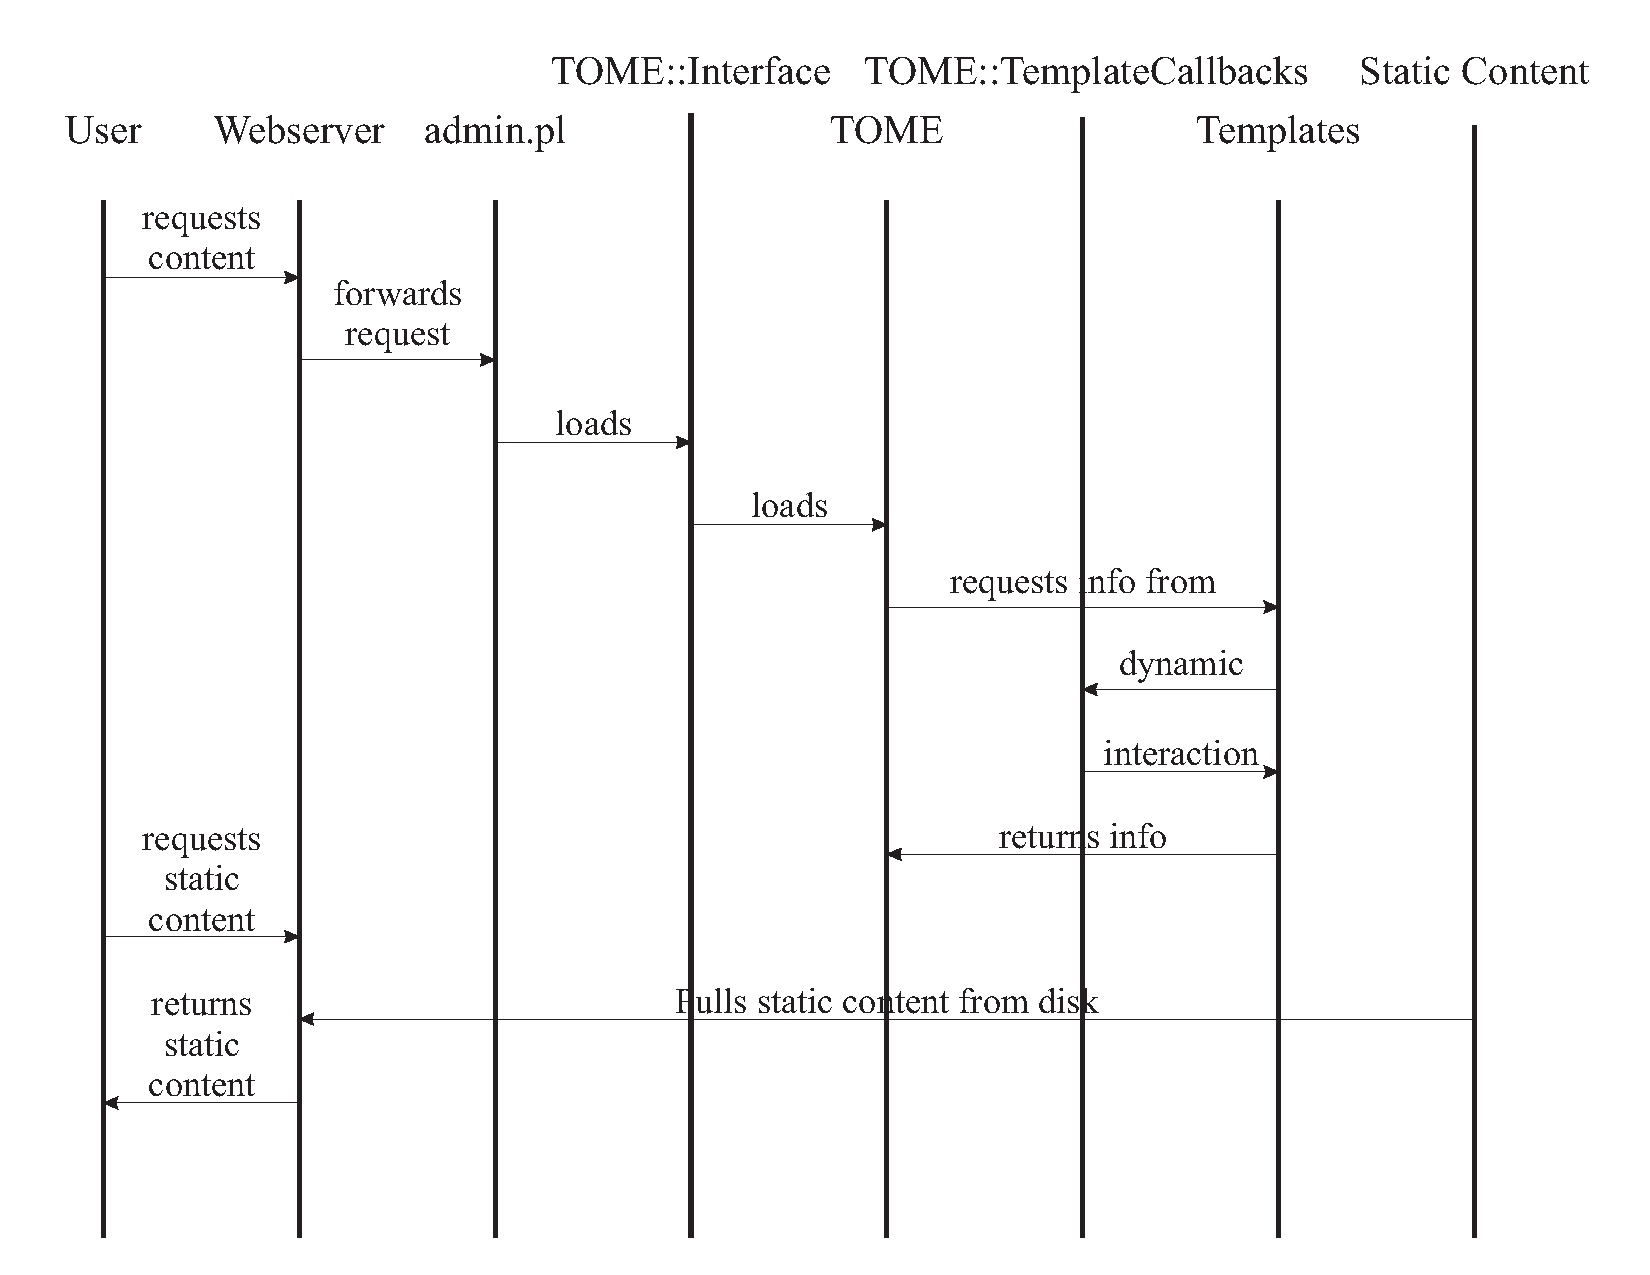
\includegraphics[width=\textwidth]{EventDiagram}
	\caption{Event Trace Diagram}
	\label{EventDiagram}
\end{figure}

\section{Component Specifications}

\subsection{admin.pl}
\subsubsection{Role}
The role of admin.pl is to load the system and serve as a starting point for the web server.
\subsubsection{Responsibilities}
admin.pl needs only to load TOME::Interface and hand control over to the CGI::Application framework.
\subsubsection{Exclusions}
admin.pl has no intrinsic understanding of anything, really.  It only hands control over to the other modules.
\subsubsection{Collaborators}
TOME::Interface collaborates very closely with admin.pl.  admin.pl loads TOME::Interface and then relinquishes control.
\subsubsection{Key Scenarios}
\paragraph{admin.pl is called by the web server}
admin.pl will load, and, in turn, load TOME::Interface.
\subsubsection{Properties}
admin.pl will be a standard text file.  It will run everything under Perl's taint mode.  It will use strict.  It will use warnings. 
\subsubsection{Creation, Existence, and Management}
admin.pl will create a single instantiation of the TOME::Interface class.  The web server (usually Apache) will be responsible for calling admin.pl.  Multiple instantiations of admin.pl (and therefore TOME::Interface and any other classes) can exist only if Apache runs multiple copies, which is expected.
\subsubsection{Resource Usage/Management}
No specific requirements exist for this component.  Resources will be limited only by the web server.
\subsubsection{State/Session/Context Management}
This component has no particular knowledge of states, sessions, or contexts.
\subsubsection{Data Storage}
This component has no intrinsic need for its own data storage.
\subsubsection{Performance}
This component does not have any specific performance or speed requirements.  Faster is better, but that is determined entirely by the machine on which it is run.  The only impact of faster or slower performance is the quality of the end user's experience.
\subsubsection{Packaging}
admin.pl is packaged as a single, executable Perl file.


\subsection{TOME::Interface}
\subsubsection{Role}
The role of TOME::Interface is to control almost all interaction between the user and TOME. Nearly every method is a CGI::Application runmode, with the exception of a few helper methods
\subsubsection{Responsibilities}
TOME::Interface is responsible for some of the set up of the CGI::Application framework.  It has all of the runmode methods that CGI::Application uses to dispatch requests served by the web server through admin.pl.  It should check all user input using the CGI::Application::Plugin::ValidateRM module.  It should also use ValidateRM's features to give good user feedback if something is wrong with their input. ValidateRM can nicely refill the form the way it was before and provide error messages.
\subsubsection{Exclusions}
TOME::Interface shouldn't know any details about the internal database structure or what things look like when they're displayed by the template.
\subsubsection{Collaborators}
TOME::Interface collaborates very closely with admin.pl.  admin.pl loads TOME::Interface and then relinquishes control.  TOME::Interface also interacts with CGI::Application::Plugin::ValidateRM to validate user input, CGI::Application::Plugin::Forward to transfer control from one runmode to another when necessary, and Crypt::PasswdMD5 to provide secure password authentication.  It also interacts with the TOME module in that it is a base class of TOME.
\subsubsection{Key Scenarios}
\paragraph{admin.pl loads TOME::Interface and calls the run method}
Since the run method is not actually a part of TOME::Interface, it has no direct responsibilities in this case.  However, the run method sets in motion a chain of events controlled by CGI::Application including calling the setup and cgiapp\_prerun methods, which are implemented by TOME::Interface.
\paragraph{A runmode dispatch occurs}
TOME::Interface contains all of the runmode subs that CGI::Application will dispatch to.  A runmode dispatch will simply run one of these methods.  When the method runs, its usual course of action will be to acquire information from the user's CGI query, make appropriate calls into the TOME core to obtain or modify database information, format that information to be used in a template, and then make the call to Template Toolkit with the appropriate information.
\subsubsection{Properties}
TOME::Interface will be a standard text file.  It will run everything under Perl's taint mode.  It will use strict.  It will use warnings. 
\subsubsection{Creation, Existence, and Management}
TOME::Interface will exist as a single instantiation created by admin.pl.  The web server (usually Apache) will be responsible for calling admin.pl.  Multiple instantiations of admin.pl (and therefore TOME::Interface and any other classes) can exist only if Apache runs multiple copies, which is expected.
\subsubsection{Resource Usage/Management}
No specific requirements exist for this component.  Resources will be limited only by the web server.
\subsubsection{State/Session/Context Management}
This component has no particular knowledge of states, sessions, or contexts.
\subsubsection{Data Storage}
This component has no intrinsic need for its own data storage.  It will interact heavily with the database, but only through the TOME module.  It has no internal knowledge of anything storage-related.
\subsubsection{Performance}
This component does not have any specific performance or speed requirements.  Faster is better, but that is determined entirely by the machine on which it is run.  The only impact of faster or slower performance is the quality of the end user's experience.
\subsubsection{Packaging}
TOME::Interface is packaged as a single Perl module name Interface.pm in the TOME directory.


\subsection{TOME}
\subsubsection{Role}
The role of the TOME module is to provide database connectivity and all utility functions used by other parts of the program.
\subsubsection{Responsibilities}
TOME needs to validate all subs with the Params::Validate module. Even if the data has already been validated inside TOME::Interface, it needs to do it again. Sooner or later, someone will make a call with unvalidated data, and catching it is critical.
\subsubsection{Exclusions}
TOME shouldn't know anything about users and especially nothing about templates.
\subsubsection{Collaborators}
TOME collaborates very closely with TOME::Interface.  TOME is the base class of TOME::Interface.  TOME is in turn implemented as a subclass of CGI::Interface.  TOME also interacts closely with several external modules such as Template Toolkit, DateTime, Params::Validate, SQL::Interpolate, CGI::Application::Plugin::DBH, CGI::Application::Plugin::Session, CGI::Application::Plugin::HTMLPrototype, and MIME::Lite.  It also uses the TOME::TemplateCallbacks modules to make dynamic callbacks available to templates.
\subsubsection{Key Scenarios}
\paragraph{TOME::Interface calls a utility method}
TOME::Interface is loaded by admin.pl and contains the runmode methods to service runmode dispatches made by CGI::Application.  In the course of servicing these requests, TOME::Interface will usually make calls to the TOME module.  These calls are handled by doing things such as interacting directly with the PostgreSQL database, interacting directly with the Template Toolkit module, or interacting directly with the MIME::Lite module to send email messages.
\paragraph{admin.pl loads TOME::Interface and calls the run method}
The TOME module also contains some of the methods that CGI::Application calls in the course of initializing itself before dispatching any runmode requests.  These include cgiapp\_init, and potentially error\_runmode.
\subsubsection{Properties}
TOME will be a standard text file.  It will run everything under Perl's taint mode.  It will use strict.  It will use warnings. 
\subsubsection{Creation, Existence, and Management}
TOME will exist as a single instantiation created by TOME::Interface when it is loaded by admin.pl.  The web server (usually Apache) will be responsible for calling admin.pl.  Multiple instantiations of admin.pl (and therefore TOME::Interface and any other classes) can exist only if Apache runs multiple copies, which is expected.
\subsubsection{Resource Usage/Management}
No specific requirements exist for this component.  Resources will be limited only by the web server.
\subsubsection{State/Session/Context Management}
This component has no particular knowledge of states, sessions, or contexts.  It does however load the CGI::Application::Plugin::Session module and configure it for use by TOME::Interface.  It also hands the current session object off to the Template Toolkit module when template calls are made.
\subsubsection{Data Storage}
This module is responsible for all interactions with the database by indirectly using the DBI module through the CGI::Application::Plugin::DBH module.  The TOME module doesn't have direct knowledge of how database operations are carried out, or especially what kind of storage mechanisms are used, but it relies upon them heavily.
\subsubsection{Performance}
This component does not have any specific performance or speed requirements.  Faster is better, but that is determined entirely by the machine on which it is run.  The only impact of faster or slower performance is the quality of the end user's experience.
\subsubsection{Packaging}
TOME is packaged as a single Perl module name TOME.pm in the modules directory.


\subsection{TOME::TemplateCallbacks}
\subsubsection{Role}
The role of the TOME::TemplateCallbacks module is to provide a way for template to dynamically request information from the TOME module.  It is used instead of a direct TOME object to increase orthogonality and prevent accident misuse of the TOME module by a template.
\subsubsection{Responsibilities}
All templates are given a "tome" object that is an instantiation of this class. The idea is that when the template is given ID numbers of various things in the database (patrons, books, tomebooks, etc.) by TOME::Interface, the template can use this object to query the database through the TOME module and get string representations of the data. This module has the place of knowing a little bit about both the template and the database. Most methods will be wrappers of TOME methods, but if there is any additional data manipulation that needs to take place before the template (without crossing the line of actually doing template work), this is the place to do it. The reason this is separate from TOME is to give an extra layer of abstraction between the actual database calls and the template.
\subsubsection{Exclusions}
This module should know a little about templates and databases, but nothing else.
\subsubsection{Collaborators}
TOME::TemplateCallbacks works closely with the TOME module.  It is passed an instantiation of it when it is instantiated itself.  It uses and interacts with no other modules.
\subsubsection{Key Scenarios}
\paragraph{A template dynamically requests information}
This information request will come through a TOME::TemplateCallbacks method.  This method will then request information from the TOME module that it has an instantiation of and return it to the template.
\paragraph{A template is generated}
All templates are generated through the TOME module, and whenever the TOME module generates a template through the Template Toolkit module, it instantiates a TOME::TemplateCallbacks object and passes it to the template.  The only important step of the instantiation is that the class is passed a reference to the current TOME object and retains it for any further calls that will be made based on dynamic information requests from the template.
\subsubsection{Properties}
TOME::TemplateCallbacks will be a standard text file.  It will run everything under Perl's taint mode.  It will use strict.  It will use warnings. 
\subsubsection{Creation, Existence, and Management}
The template method within the TOME module is responsible for instantiating all instances of the TOME::TemplateCallbacks module.  Usually, there will only be one template created per TOME instance, but in some cases, such as when emails are sent out using templates, there may be multiple template objects created.  This will not cause any problems.
\subsubsection{Resource Usage/Management}
No specific requirements exist for this component.  Resources will be limited only by the web server.
\subsubsection{State/Session/Context Management}
This component has no particular knowledge of states, sessions, or contexts.
\subsubsection{Data Storage}
This module has no intrinsic data storage requirements.
\subsubsection{Performance}
This component does not have any specific performance or speed requirements.  Faster is better, but that is determined entirely by the machine on which it is run.  The only impact of faster or slower performance is the quality of the end user's experience.
\subsubsection{Packaging}
TOME is packaged as a single Perl module name TemplateCallbacks.pm in the TOME directory.


\subsection{Templates}
\subsubsection{Role}
The role of the templates is to control the actual presentation of data by determining the HTML representation of the information gathered by TOME::Interface and TOME::TemplateCallbacks from TOME.  These are HTML-style files that are interpreted by the Template Toolkit module; they are not an actual class.
\subsubsection{Responsibilities}
Structures that are used commonly should be put in the blocks directory and INCLUDEd in the other templates. INCLUDE can take a list of locally-scoped variables, which essentially makes the files in blocks like little subroutines.
\subsubsection{Exclusions}
The templates should be as free as possible from any knowledge about the database or any internals of the TOME system.
\subsubsection{Collaborators}
Templates are retrieved by the TOME module, usually at the behest of the TOME::Interface module.  The only way the templates have to interact with the other system in an active manner is through the TOME::TemplateCallbacks module.  The templates neither know how they have been called nor what will be done with the information they synthesize.
\subsubsection{Key Scenarios}
\paragraph{A template dynamically requests information}
This information request will come through a TOME::TemplateCallbacks method.  This method will then request information from the TOME module that it has an instantiation of and return it to the template.
\paragraph{A template is generated}
The template's HTML-style information will be interpreted by the Template Toolkit library.
\subsubsection{Properties}
These are plain text files.  They do not really execute code, only provide direction for the Template Toolkit library.
\subsubsection{Creation, Existence, and Management}
As these are not classes, they are not ever instantiated.  They are loaded by the TOME module, usually as a response to a request by the TOME::Interface module.
\subsubsection{Resource Usage/Management}
No specific requirements exist for this component.  Resources will be limited only by the web server.
\subsubsection{State/Session/Context Management}
This component has no particular knowledge of states, sessions, or contexts.  It can, however, access information about the current session based on a session object passed to it by the TOME module.
\subsubsection{Data Storage}
This module has no intrinsic data storage requirements.
\subsubsection{Performance}
This component does not have any specific performance or speed requirements.  Faster is better, but that is determined entirely by the machine on which it is run.  The only impact of faster or slower performance is the quality of the end user's experience.
\subsubsection{Packaging}
The templates are plain text files located in the templates directory.


\subsection{Static Content}
\subsubsection{Role}
The role of the static content is to serve as a location for any content that does not have to be dynamically generated for every call to the TOME system.  Examples include logo graphics, static CSS files, and static Javascript files.
\subsubsection{Responsibilities}
The only responsibilities for this component are to be correctly formatted and up to date.
\subsubsection{Exclusions}
These files cannot be expected to by dynamically generated in any case.
\subsubsection{Collaborators}
These files will be called by the output of templates by the user's web browser and retrieved by the web server.
\subsubsection{Key Scenarios}
\paragraph{A template contains information that will request a static file}
The user's web browser will recognize the request, pass it on to the webserver, the webserver will return the file, and the browser will interpret it.
\subsubsection{Properties}
These are plain text files.  They do not really execute code, only provide various static content.
\subsubsection{Creation, Existence, and Management}
As these are not classes, they are not ever instantiated.  They are loaded by the user's web browser when needed, usually because the output of a template requests them.
\subsubsection{Resource Usage/Management}
No specific requirements exist for this component.  Resources will be limited only by the web server.
\subsubsection{State/Session/Context Management}
This component has no particular knowledge of states, sessions, or contexts.
\subsubsection{Data Storage}
This module has no intrinsic data storage requirements.
\subsubsection{Performance}
This component does not have any specific performance or speed requirements.  Faster is better, but that is determined entirely by the machine on which it is run.  The only impact of faster or slower performance is the quality of the end user's experience.
\subsubsection{Packaging}
The static content is plain text files located in the static directory.

\section{Class Interfaces}
Note: up-to-date documentation of the entire interface is always available by viewing the POD embedded in any of the Perl modules for this project.  The following is the core interface for the TOME class.

\subsection{CONFIG}
The CONFIG hash describes various and sundry configurata.

These configurata are:
\paragraph{cgibase}
the relative location of the cgi stuff 

\paragraph{staticbase}
the relative location of the static stuff 

\paragraph{templatepath}
the relative location of the templates 

\paragraph{dbidbname}
the database name that TOME is stored under 

\paragraph{dbihostname}
the hostname of the database server 

\paragraph{dbiport}
the port the database server is running on 

\paragraph{dbiusername}
username for the database 

\paragraph{dbipassword}
password for the database 

\paragraph{notifyfrom}
the address email messages are from 

\paragraph{adminemail}
the address email messages are sent to 

\paragraph{devmode}
whether or not this is being run in development mode 

\paragraph{devemailto}
the address email messages are sent to when in development mode 

Note: address format is 'Name <email@domain>`

\subsection{cgiapp_init}
This sets up various variables that are needed for CGI stuff. It takes no arguments.

\subsection{error_runmode}
This is called when there is an error that we really don't know what caused. This takes one argument:

\paragraph{error}
the error message

\subsection{error}
This function is called when there is a fatal error.

This function takes a hash as an argument:
\paragraph{message}
the short error message 

\paragraph{extended}
the details of the error message

\subsection{tomebooks_search}
This returns an array of found textbooks.

It takes arguments in the form of a hash:
\paragraph{isbn}
the isbn to look for 

\paragraph{status}
that status of the book (all, can_reserve, can_checkout, or in_collection) 

\paragraph{title}
the title of the book 

\paragraph{author}
the author of the book 

\paragraph{edition}
the edition of the book 

\paragraph{libraries}
the libraries to look in for the book

\paragraph{semester}
the semester that the book is here for

\subsection{expire_search}
This function returns a list of books that will expire on the given semester with the given libraries.

The arguments are given as a hash:
\paragraph{semester}
The semester in which the books will expire 

\paragraph{libraries}
The libraries the books reside in

\subsection{reservation_search}
This function returns an array of books that are reserved in a given semester from given libraries.

The arguments are given as a hash:
\paragraph{semester}
the semester that the books are reserved for 

\paragraph{libraries}
the libraries that the books are in

\subsection{dueback_search}
This function returns a list of books that are due back at the given semester from the given libraries.

The arguments are given as a hash:
\paragraph{semester}
the semester that the books are due back 

\paragraph{libraries}
the libraries that the books are in

\subsection{add_book}
This function is used to add a book to TOME. This is not for adding a real book, but for adding a book type. Like adding a Class, not an Object.

This function takes a hash as an argument:
\paragraph{isbn}
The ISBN of the book 

\paragraph{title}
The Title of the book 

\paragraph{author}
The Author of the book 

\paragraph{edition}
The Edition of the book

\subsection{add_class}
This function adds a class to TOME.

The arguments are given as a hash:
\paragraph{id}
The "School Readable" name of the class (that is, something like, MATH9999) 

\paragraph{name}
The Human Readable name of the Class

\subsection{patrons_search}
This function finds patrons.

Arguments are given as a hash:
\paragraph{id}
The numeric, databasical id of the patron 

\paragraph{name}
The Real Name of the patron 

\paragraph{email}
The Email of the patron

\subsection{patron_add}
This function adds a patron to the database.

This function takes arguments as a hash as follows:
\paragraph{email}
The email address of the patron 

\paragraph{name}
The name of the patron (Often the patron's nickname)

\subsection{patron_update}
This function changes the patron at a given id.

The arguments to this function are given as a hash, as usual:
\paragraph{id}
The id of the patron to change 

\paragraph{email}
The email to set for the given id 

\paragraph{name}
The name to set to the given id

\subsection{patron_info}
This function returns information about patrons matching certain critereon.

The function looks for the following to parameters in a hash in this order:
\paragraph{email}
The email to try to find 

\paragraph{id}
The exact id to find

\subsection{patron_classes}
This function finds the classes associated with a patron for a given semester.

Arguments are given as a hash:
\paragraph{patron}
The numeric, databasical id of the patron 

\paragraph{semester}
The ID of the semester to retrieve classes for. 

Returns: An arrayref containing class ids.

\subsection{patron_add_class}
This function adds a class associated with a patron for a given semester.

Arguments are given as a hash:
\paragraph{patron}
The numeric, databasical id of the patron 

\paragraph{semester}
The ID of the semester to retrieve classes for. 

\paragraph{class}
The ID of the class to add. 

Returns: Nothing.

\subsection{patron_delete_class}
This function deletes a class associated with a patron for a given semester.

Arguments are given as a hash:
\paragraph{patron}
The numeric, databasical id of the patron 

\paragraph{semester}
The ID of the semester to retrieve classes for. 

\paragraph{class}
The ID of the class to add. 

Returns: Nothing.

\subsection{class_info}
This method returns information about class

Arguments are given as a hash:
\paragraph{id}
The numeric, databasical id of the class 

Returns a hash:
\paragraph{name}
The text name of the class 

\paragraph{comments}
The text comments about the class 

\paragraph{verified}
Semester ID for which the class has been verified. 

\paragraph{uid}
User ID of the TOMEkeeper that did the last verification

\subsection{class_books}
This method returns books associated with a class

Arguments are given as a hash:
\paragraph{id}
The numeric, databasical id of the class 

Returns an arrayref to an array of hashrefs:
\paragraph{isbn}
ISBN of the book 

\paragraph{verified}
Semester ID for when the book was last verified 

\paragraph{comments}
Comments about the verification of the book 

\paragraph{usable}
Boolean indicating if the book is usable or not 

\paragraph{uid}
The user id of the TOMEkeeper who did the verification

\subsection{class_update_verified}
This method upates information about a class

Arguments are given as a hash:
\paragraph{id}
The numeric, databasical id of the class 

\paragraph{verified}
The ID of the semester for which the class has been verified 

\paragraph{uid}
The ID of the TOMEkeeper that did the verification 

Returns nothing.



\section{Component Design}
\subsection{Pattern Usage}
TOME is built around an MVC pattern.  The Model is handled by the TOME model, the View is handled by the templates, and the Control is handled by TOME::Interface.
\subsection{Limitations}
One major limitation of the current design is that TOME::Interface inherits from TOME.  This introduces both namespace pollution and fragile base class issues.  However, after assessing the benefits of moving to a delegation approach versus coping with the current approach, it was determined that, for now, we will continue with the existing design, limited as it may be.


\section{Class Diagram}
The class diagram for the TOME system can be seen in Figure~\ref{ComponentDiagram}.
\begin{figure}[h]
	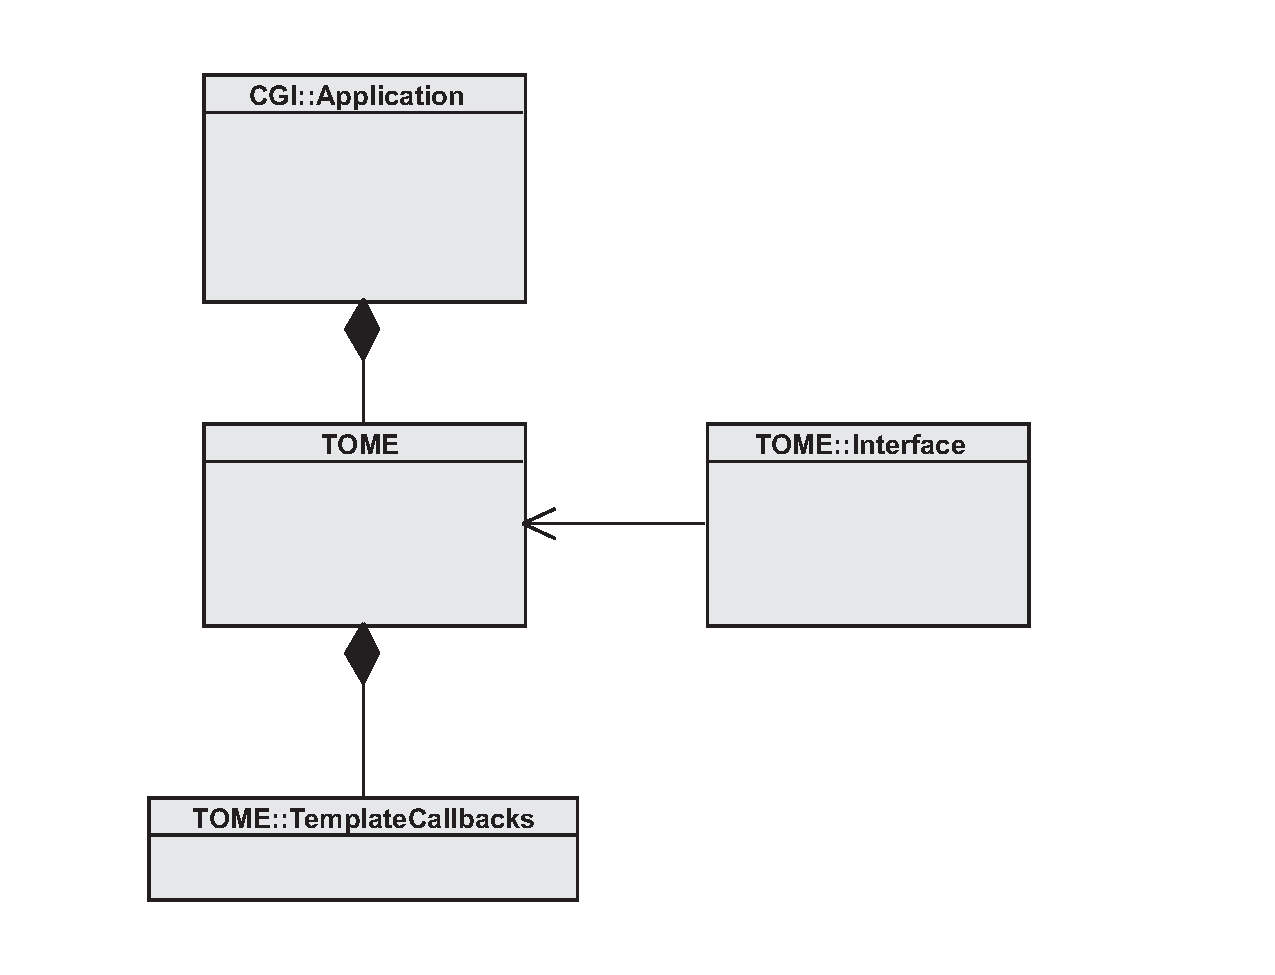
\includegraphics[width=\textwidth]{ComponentDiagram}
	\caption{Class Diagram}
	\label{ComponentDiagram}
\end{figure}


\section{Database Structure}
\label{tomedbsection}
The overall structure of the database can be seen in Figure~\ref{tomedb}.  In addition to the structure, there are also triggers that ensure the consistency of the database at all times.
\begin{figure}[h]
	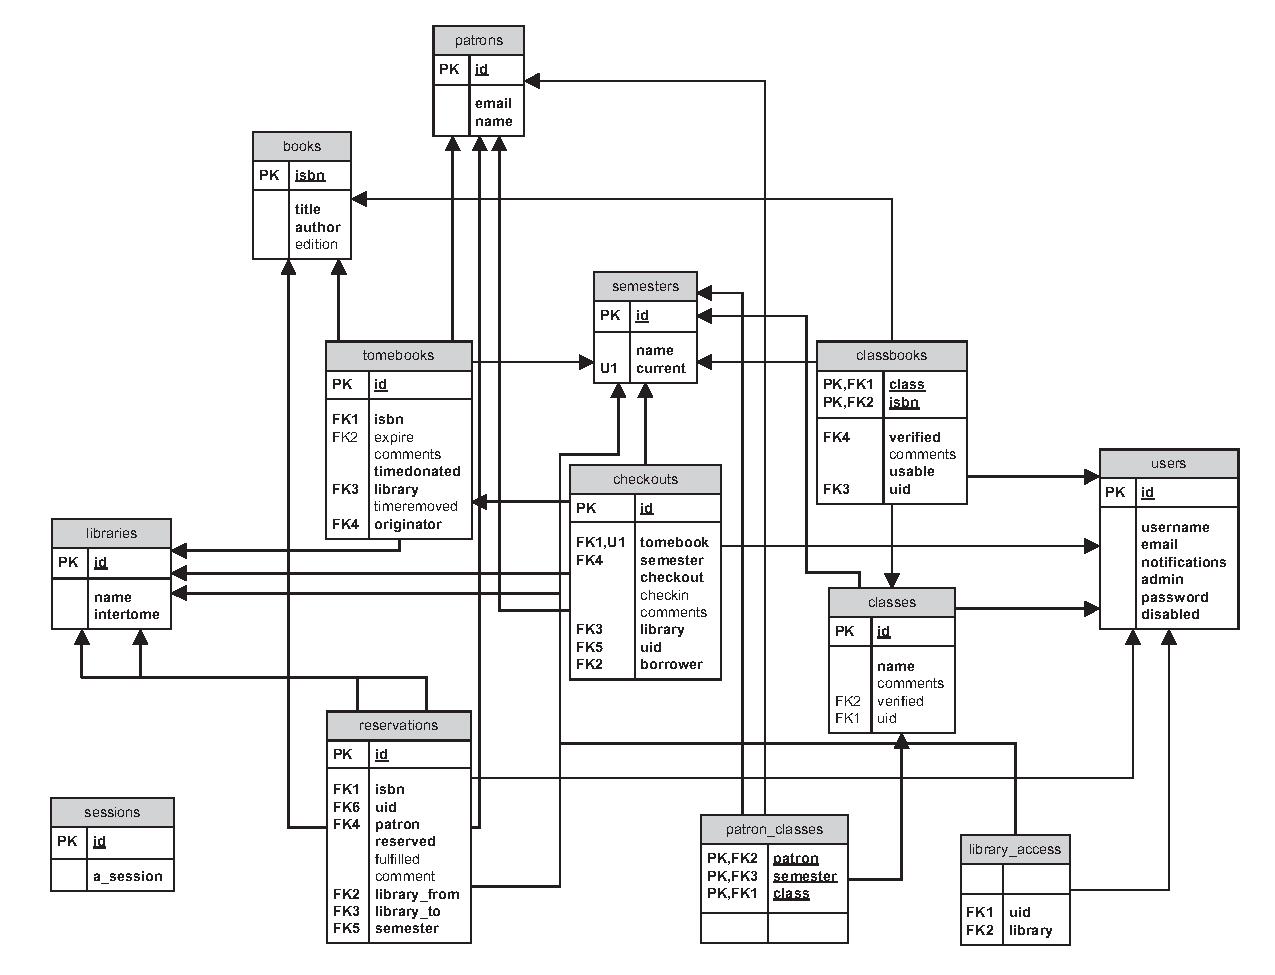
\includegraphics[width=\textwidth]{tomedb}
	\caption{Database Diagram}
	\label{tomedb}
\end{figure}

\end{document}

